%%% Copyright (C) 2018 Vincent Goulet
%%%
%%% Ce fichier fait partie du projet
%%% «Méthodes numériques en actuariat avec R»
%%% http://github.com/vigou3/methodes-numeriques-en-actuariat
%%%
%%% Cette création est mise à disposition selon le contrat
%%% Attribution-Partage dans les mêmes conditions 4.0
%%% International de Creative Commons.
%%% http://creativecommons.org/licenses/by-sa/4.0/

\documentclass[letterpaper,11pt,x11names,english,french]{memoir}
  \usepackage{natbib,url}
  \usepackage{babel}
  \usepackage[autolanguage]{numprint}
  \usepackage{amsmath,amsthm}
  \usepackage[noae]{Sweave}
  \usepackage{graphicx}
  \usepackage{actuarialangle}          % \angl et al.
  \usepackage{framed}                  % env. snugshade*, oframed
  \usepackage{paralist}
  \usepackage[shortlabels]{enumitem}   % configuration listes
  \usepackage[absolute]{textpos}       % éléments des pages de titre
  \usepackage{relsize}                 % \smaller et al.
  \usepackage{manfnt}                  % \mantriangleright (puce)
  \usepackage{metalogo}                % \XeLaTeX logo
  \usepackage{fontawesome}             % icônes \fa*
  \usepackage{awesomebox}              % boites info, important, etc.
  \usepackage{answers}                 % exercices et solutions
  \usepackage{listings}                % code informatique
  \usepackage{xr}                      % références entre parties

  %%% =======================================================
  %%%  Informations de publication (sauf titre de la partie)
  %%% =======================================================
  \title{Méthodes numériques en actuariat avec R}
  \author{Vincent Goulet}
  \renewcommand{\year}{2018}
  \renewcommand{\month}{01}
  \newcommand{\ghurl}{https://github.com/vigou3/methodes-numeriques-en-actuariat/}

  %%% ===================
  %%%  Style du document
  %%% ===================

  %% Polices de caractères
  \usepackage{fontspec}
  \usepackage[bold-style=upright]{unicode-math}
  \defaultfontfeatures{Scale=0.92}
  \setmainfont[Ligatures=TeX,Numbers=OldStyle]{Lucida Bright OT}
  \setmathfont{Lucida Bright Math OT}
  \setmonofont{Lucida Grande Mono DK}
  \setsansfont[Scale=1.0,Numbers=OldStyle]{Myriad Pro}
  \newfontfamily\fullcaps[Letters=Uppercase,Numbers=Uppercase]{Myriad Pro}
  \usepackage[babel=true]{microtype}
  \usepackage{icomma}

  %% Couleurs
  \usepackage{xcolor}
  \definecolor{comments}{rgb}{0.7,0,0}           % commentaires
  \definecolor{link}{rgb}{0,0.4,0.6}             % liens internes
  \definecolor{url}{rgb}{0.6,0,0}                % liens externes
  \definecolor{citation}{rgb}{0,0.5,0}           % citations
  \definecolor{codebg}{named}{LightYellow1}      % fond code R
  \definecolor{prob}{named}{orange}              % encadrés «problème»
  \definecolor{rouge}{rgb}{0.85,0,0.07} % rouge bandeau identitaire
  \definecolor{or}{rgb}{1,0.8,0}        % or bandeau identitaire

  %% Hyperliens
  \usepackage{hyperref}
  \hypersetup{%
    pdfauthor = {Vincent Goulet},
    colorlinks = {true},
    linktocpage = {true},
    urlcolor = {url},
    linkcolor = {link},
    citecolor = {citation},
    pdfpagemode = {UseOutlines},
    pdfstartview = {Fit},
    bookmarksopen = {true},
    bookmarksnumbered = {true},
    bookmarksdepth = {subsubsection}}
  \setlength{\XeTeXLinkMargin}{1pt}

  %% Étiquettes de \autoref (redéfinitions compatibles avec babel).
  %% Attention! Les % à la fin des lignes sont importants sinon des
  %% blancs apparaissent dès que la commande \selectlanguage est
  %% utilisée... comme dans la bibliographie, par exemple.
  \addto\extrasfrench{%
    \def\algorithmeautorefname{algorithme}%
    \def\appendixautorefname{annexe}%
    \def\definitionautorefname{définition}%
    \def\figureautorefname{figure}%
    \def\exempleautorefname{exemple}%
    \def\exerciceautorefname{exercice}%
    \def\subfigureautorefname{figure}%
    \def\subsectionautorefname{section}%
    \def\subtableautorefname{tableau}%
    \def\tableautorefname{tableau}%
    \def\thmautorefname{théorème}%
  }

  %% Table des matières (inspirée de classicthesis.sty)
  \renewcommand{\cftchapterleader}{\hspace{1.5em}}
  \renewcommand{\cftchapterafterpnum}{\cftparfillskip}
  \renewcommand{\cftsectionleader}{\hspace{1.5em}}
  \renewcommand{\cftsectionafterpnum}{\cftparfillskip}

  %% Titres des chapitres
  \chapterstyle{hangnum}
  \renewcommand{\chaptitlefont}{\normalfont\Huge\sffamily\bfseries\raggedright}

  %% Marges, entêtes et pieds de page
  \setlength{\marginparsep}{7mm}
  \setlength{\marginparwidth}{13mm}
  \setlength{\headwidth}{\textwidth}
  \addtolength{\headwidth}{\marginparsep}
  \addtolength{\headwidth}{\marginparwidth}

  %% Titres des sections et sous-sections
  \setsecheadstyle{\normalfont\Large\sffamily\bfseries\raggedright}
  \setsubsecheadstyle{\normalfont\large\sffamily\bfseries\raggedright}
  \maxsecnumdepth{subsection}
  \setsecnumdepth{subsection}

  %% Listes. Paramétrage avec enumitem.
  \setlist[enumerate]{leftmargin=*,align=left}
  \setlist[enumerate,2]{label=\alph*),labelsep=*,leftmargin=1.5em}
  \setlist[enumerate,3]{label=\roman*),labelsep=*,leftmargin=1.5em,align=right}
  \setlist[itemize]{leftmargin=*,align=left}

  %% Options de babel
  \frenchbsetup{StandardItemizeEnv=true,%
    ThinSpaceInFrenchNumbers=true,
    ItemLabeli=\mantriangleright,
    ItemLabelii=\textendash,
    og=«, fg=»}
  \addto\captionsfrench{\def\figurename{{\scshape Fig.}}}
  \addto\captionsfrench{\def\tablename{{\scshape Tab.}}}

  %% Sections de code source
  \lstloadlanguages{R}
  \lstset{language=R,
    basicstyle=\small\ttfamily\NoAutoSpacing,
    keywordstyle=\mdseries,
    commentstyle=\color{comments}\slshape,
    extendedchars=true,
    showstringspaces=false}

  %%% =========================
  %%%  Nouveaux environnements
  %%% =========================

  %% Environnements d'exemples et al.
  \theoremstyle{plain}
  \newtheorem{algorithme}{Algorithme}[chapter]
  \newtheorem{thm}{Théorème}[chapter]

  \theoremstyle{definition}
  \newtheorem{exemple}{Exemple}[chapter]
  \newtheorem{definition}{Définition}[chapter]
  \newtheorem*{astuce}{Astuce}

  \theoremstyle{remark}
  \newtheorem*{remarque}{Remarque}
  \newtheorem*{remarques}{Remarques}
  \newenvironment{rem}{\begin{remarque} \mbox{}}{\end{remarque}}
  \newenvironment{rems}{\begin{remarques} \mbox{}}{\end{remarques}}

  %% Redéfinition de l'environnement titled-frame de framed.sty avec
  %% deux modifications: épaisseur des filets réduite de 2pt à 1pt;
  %% "(suite)" plutôt que "(cont)" dans la barre de titre
  %% lorsque l'encadré se poursuit après un saut de page.
  \renewenvironment{titled-frame}[1]{%
    \def\FrameCommand{\fboxsep8pt\fboxrule1pt
      \TitleBarFrame{\textbf{#1}}}%
    \def\FirstFrameCommand{\fboxsep8pt\fboxrule1pt
      \TitleBarFrame[$\blacktriangleright$]{\textbf{#1}}}%
    \def\MidFrameCommand{\fboxsep8pt\fboxrule1pt
      \TitleBarFrame[$\blacktriangleright$]{\textbf{#1\ (suite)}}}%
    \def\LastFrameCommand{\fboxsep8pt\fboxrule1pt
      \TitleBarFrame{\textbf{#1\ (suite)}}}%
    \MakeFramed{\advance\hsize-16pt \FrameRestore}}%
  {\endMakeFramed}

  %% Encadré générique avec titre basé sur titled-frame, ci-dessus.
  %% Sert pour les listes d'objectifs et les encadrés reliés aux
  %% problèmes (mises en situation) dans les chapitres. Arguments:
  %% couleur du cadre (optionnel; noir par défaut) et titre de la
  %% boîte (obligatoire).
  \newenvironment{emphbox}[2][black]{%
    \colorlet{TFFrameColor}{#1}%
    \colorlet{TFTitleColor}{white}%
    \begin{titled-frame}{\sffamily #2}%
      \setlength{\parindent}{0pt}}%
    {\end{titled-frame}}

  %% Liste d'objectifs au début des chapitres
  \newenvironment{objectifs}{%
    \begin{emphbox}{\rule[-7pt]{0pt}{20pt} Objectifs du chapitre}
      \begin{itemize}[nosep]
        \small\sffamily}%
      {\end{itemize}\end{emphbox}}

  %% Problèmes (mises en situation) des chapitres: énoncé au début du
  %% chapitre; astuces en cours de chapitre; solution à la fin
  %% du chapitre.
  \newenvironment{prob-enonce}{%
    \begin{emphbox}[prob]{{\normalfont\faCogs}\; Énoncé du problème}}%
    {\end{emphbox}}
  \newenvironment{prob-astuce}{%
    \begin{emphbox}[prob]{{\normalfont\faBolt}\; Astuce}}%
    {\end{emphbox}}
  \newenvironment{prob-solution}{%
    \begin{emphbox}[prob]{{\normalfont\faLightbulbO}\; Solution du problème}}%
    {\end{emphbox}}

  %% Environnements de Sweave. Les environnements Sinput et Soutput
  %% utilisent Verbatim (de fancyvrb). On les réinitialise pour
  %% enlever la configuration par défaut de Sweave, puis on réduit
  %% l'écart entre les blocs Sinput et Soutput.
  \DefineVerbatimEnvironment{Sinput}{Verbatim}{}
  \DefineVerbatimEnvironment{Soutput}{Verbatim}{}
  \fvset{listparameters={\setlength{\topsep}{0pt}}}

  %% L'environnement Schunk est complètement redéfini en un hybride
  %% des environnements snugshade* et leftbar de framed.sty.
  \makeatletter
  \renewenvironment{Schunk}{%
    \setlength{\topsep}{1pt}
    \def\FrameCommand##1{\hskip\@totalleftmargin
       \vrule width 2pt\colorbox{codebg}{\hspace{3pt}##1}%
      % There is no \@totalrightmargin, so:
      \hskip-\linewidth \hskip-\@totalleftmargin \hskip\columnwidth}%
    \MakeFramed {\advance\hsize-\width
      \@totalleftmargin\z@ \linewidth\hsize
      \advance\labelsep\fboxsep
      \@setminipage}%
  }{\par\unskip\@minipagefalse\endMakeFramed}
  \makeatother

  %% Exercices et réponses
  \Newassociation{sol}{solution}{solutions}
  \Newassociation{rep}{reponse}{reponses}
  \newcounter{exercice}[chapter]
  \renewcommand{\theexercice}{\thechapter.\arabic{exercice}}
  \newenvironment{exercice}[1][]{%
    \begin{list}{}{%
        \refstepcounter{exercice}
        \ifthenelse{\equal{#1}{nosol}}{%
          \renewcommand{\makelabel}{\bfseries\theexercice}}{%
          \hypertarget{ex:\theexercice}{}
          \Writetofile{solutions}{\protect\hypertarget{sol:\theexercice}{}}
          \renewcommand{\makelabel}{%
            \bfseries\protect\hyperlink{sol:\theexercice}{\theexercice}}}
        \settowidth{\labelwidth}{\bfseries\theexercice}
        \setlength{\leftmargin}{\labelwidth}
        \addtolength{\leftmargin}{\labelsep}
        \setlist[enumerate,1]{label=\alph*),labelsep=*,leftmargin=1.5em}
        \setlist[enumerate,2]{label=\roman*),labelsep=0.5em,align=right}}
      \item}%
      {\end{list}}
  \renewenvironment{solution}[1]{%
    \begin{list}{}{%
        \renewcommand{\makelabel}{%
          \bfseries\protect\hyperlink{ex:#1}{#1}}
        \settowidth{\labelwidth}{\bfseries #1}
        \setlength{\leftmargin}{\labelwidth}
        \addtolength{\leftmargin}{\labelsep}
        \setlist[enumerate,1]{label=\alph*),labelsep=*,leftmargin=1.5em}
        \setlist[enumerate,2]{label=\roman*),labelsep=0.5em,align=right}}
    \item}%
    {\end{list}}
  \renewenvironment{reponse}[1]{%
    \begin{enumerate}[label=\textbf{#1}]
    \item}%
    {\end{enumerate}}

  %% Redéfinition de l'environnement de matrices de amsmath pour
  %% aligner les colonnes à droite. Pris dans
  %% <http://texblog.net/latex-archive/maths/matrix-align-left-right/>
  \makeatletter
  \renewcommand*\env@matrix[1][r]{\hskip -\arraycolsep
    \let\@ifnextchar\new@ifnextchar
    \array{*\c@MaxMatrixCols #1}}
  \makeatother

  %%% =====================
  %%%  Nouvelles commandes
  %%% =====================

  %% Noms de fonctions, code, etc.
  \newcommand{\code}[1]{\texttt{#1}}
  \newcommand{\pkg}[1]{\textbf{#1}}

  %% Hyperlien avec symbole de lien externe juste après; second
  %% argument peut être vide pour afficher l'url comme lien
  %% [https://tex.stackexchange.com/q/53068/24355 pour procédure de
  %% test du second paramètre vide]
  \newcommand{\link}[2]{%
    \def\param{#2}%
    \ifx\param\empty
      \href{#1}{\nolinkurl{#1}~\raisebox{-0.1ex}{\smaller\faExternalLink}}%
    \else
      \href{#1}{#2~\raisebox{-0.1ex}{\smaller\faExternalLink}}%
    \fi
  }

  %% Indications de capsule vidéo
  \newcommand{\capsule}[2]{\href{#1}{#2}\marginpar{%
      \href{#1}{\raisebox{-0.5em}[0em][0em]{\HUGE\faYoutubePlay}}}}

  %% Boites additionnelles (basées sur awesomebox.sty) pour remarques
  %% spécifiques à macOS et pour les changements au fil de la lecture.
  \newcommand{\osxbox}[1]{%
    \awesomebox{\faApple}{\aweboxrulewidth}{black}{#1}}
  \newcommand{\gotorbox}[1]{%
    \awesomebox{\faMapSigns}{\aweboxrulewidth}{black}{\sffamily #1}}

  %% Boite pour le nom du fichier de script correspondant au début des
  %% sections d'exemples.
  \newcommand{\scriptfile}[1]{%
    \begingroup
    \noindent
    \mbox{%
      \makebox[3mm][l]{\raisebox{-0.5pt}{\small\faChevronCircleDown}}\;%
      \smaller[1] {\sffamily Fichier d'accompagnement} {\ttfamily #1}}
    \endgroup}

  %% Lien vers GitHub dans la page de notices
  \newcommand{\viewsource}[1]{%
    \href{#1}{%
      Voir sur GitHub \raisebox{-1pt}{\footnotesize\faGithub}}}

  %% Raccourcis usuels vg
  \newcommand{\pt}{{\scriptscriptstyle \Sigma}}
  \newcommand{\abs}[1]{\lvert #1 \rvert}
  \newcommand{\norme}[1]{\lVert #1 \rVert}
  \newcommand{\mat}[1]{\symbf{#1}}
  \newcommand{\diag}{\operatorname{diag}}
  \newcommand{\Esp}[1]{E\! \left[ #1 \right]}
  \newcommand{\esp}[1]{E [ #1 ]}
  \newcommand{\Var}[1]{\operatorname{Var}\! \left[ #1 \right]}
  \newcommand{\var}[1]{\operatorname{Var} [ #1 ]}
  \newcommand{\Prob}[1]{\operatorname{Pr}\! \left[ #1 \right]}
  \newcommand{\prob}[1]{\operatorname{Pr} [ #1 ]}
  \newcommand{\R}{\symbb{R}}    % ensemble des réels

  %% Traitement du titre de partie
  \makeatletter
  \newcommand{\@parttitle}{}
  \newcommand{\parttitle}[1]{\renewcommand{\@parttitle}{#1}}
  \newcommand{\theparttitle}{\@parttitle}
  \makeatother

  %%% =======
  %%%  Varia
  %%% =======

  %% Sous-tableaux et figures
  \newsubfloat{table}
  \newsubfloat{figure}

  %% Style de la bibliographie
  \bibliographystyle{francais}

  %% Longueurs pour la composition des pages couvertures avant et
  %% arrière.
  \newlength{\banderougewidth} \newlength{\banderougeheight}
  \newlength{\bandeorwidth}    \newlength{\bandeorheight}
  \newlength{\imageheight}
  \newlength{\logoheight}
  \newlength{\gapwidth}

  %% Aide pour la césure
  \hyphenation{%
    con-gru-en-tiels
    con-naî-tre
    con-sole
    cons-tante
    con-tenu
    con-trôle
    hexa-dé-ci-mal
    nom-bre
    puis-que
  }

  \usepackage{wasysym}         % \leadsto

  %%%  Titre du document
  \parttitle{%
    \bfseries\fontsize{36}{36}\selectfont Partie I \\
    \mdseries\fontsize{32}{36}\selectfont Programmation en R}
  \hypersetup{pdftitle={Méthodes numériques en actuariat - Partie I
      Programmation en R}}

  %%% Listes de commandes
  \newenvironment{ttscript}[1]{%
    \begin{list}{}{%
        \setlength{\labelsep}{1.5ex}
        \settowidth{\labelwidth}{\fbox{\code{#1}}}
        \setlength{\leftmargin}{\labelwidth}
        \addtolength{\leftmargin}{\labelsep}
        \setlength{\parsep}{0.5ex plus0.2ex minus0.2ex}
        \setlength{\itemsep}{0.3ex}
        \renewcommand{\makelabel}[1]{\fbox{\vphantom{|}##1}\hfill}}}
    {\end{list}}

  %%% Chapitre Opérateurs: environnements pour placer côte à côte des
  %%% définitions de fonctions (utilisant ttscript ci-dessus) et un
  %%% petit exemple.
  \newenvironment{operateur}[1]{%
    \noindent
    \begin{minipage}[t]{0.65\linewidth}
      \begin{ttscript}{#1}}
    {\end{ttscript}\end{minipage}\hfill}
  \newenvironment{miniexemple}{%
    \begin{minipage}[t]{0.3\linewidth}}
    {\end{minipage}}

  %%% Listes de structures de contrôle
  \newenvironment{struclist}{%
    \begin{description}[style=nextline,font=\mdseries\ttfamily]}
    {\end{description}}

  %%% Paramètres additionels pour sections de code source
  \lstdefinelanguage{Renhanced}[]{R}{%
    morekeywords={colMeans,colSums,head,is.na,is.null,mapply,ms,na.rm,%
      nlmin,replicate,row.names,rowMeans,rowSums,sys.time,system.time,%
      tail,which.max,which.min},
    deletekeywords={c},
    alsoletter={.\%},%
    alsoother={:_\$}}
  \lstset{language=Renhanced,
    index=[1][keywords],
    indexstyle=\indexfonction}

  %%% Index
  \newcommand{\bfhyperpage}[1]{\textbf{\hyperpage{#1}}}
  \renewcommand{\preindexhook}{%

    Les numéros de page en caractères gras indiquent les pages où les
    concepts sont introduits, définis ou expliqués.\vskip\onelineskip}
  \newcommand{\Index}[1]{\index{#1|bfhyperpage}}
  \newcommand{\indexargument}[1]{\index{#1@\code{#1}}}
  \newcommand{\Indexargument}[1]{\Index{#1@\code{#1}}}
  \newcommand{\indexattribut}[1]{\index{#1@\code{#1} (attribut)}}
  \newcommand{\Indexattribut}[1]{\Index{#1@\code{#1} (attribut)}}
  \newcommand{\indexclasse}[1]{\index{#1@\code{#1} (classe)}}
  \newcommand{\Indexclasse}[1]{\Index{#1@\code{#1} (classe)}}
  \newcommand{\indexfonction}[1]{\index{#1@\code{#1}}}
  \newcommand{\Indexfonction}[1]{\Index{#1@\code{#1}}}
  \newcommand{\indexmode}[1]{\index{#1@\code{#1} (mode)}}
  \newcommand{\Indexmode}[1]{\Index{#1@\code{#1} (mode)}}
  \newcommand{\indexobjet}[1]{\index{#1@\code{#1}}}
  \newcommand{\Indexobjet}[1]{\Index{#1@\code{#1}}}
  \newcommand{\indexemacs}[1]{\index{Emacs!#1@\texttt{#1}}}
  \newcommand{\indexess}[1]{\index{ESS!#1@\texttt{#1}}}

  \newcommand{\attribut}[1]{\code{#1}\indexattribut{#1}}
  \newcommand{\Attribut}[1]{\code{#1}\Indexattribut{#1}}
  \newcommand{\argument}[1]{\code{#1}\indexargument{#1}}
  \newcommand{\Argument}[1]{\code{#1}\Indexargument{#1}}
  \newcommand{\classe}[1]{\code{#1}\indexclasse{#1}}
  \newcommand{\Classe}[1]{\code{#1}\Indexclasse{#1}}
  \newcommand{\fonction}[1]{\code{#1}\indexfonction{#1}}
  \newcommand{\Fonction}[1]{\code{#1}\Indexfonction{#1}}
  \newcommand{\mode}[1]{\code{#1}\indexmode{#1}}
  \newcommand{\Mode}[1]{\code{#1}\Indexmode{#1}}
  \newcommand{\objet}[1]{\code{#1}\indexobjet{#1}}
  \newcommand{\Objet}[1]{\code{#1}\Indexobjet{#1}}
  \newcommand{\emacs}[1]{\code{#1}\indexemacs{#1}}
  \newcommand{\ess}[1]{\code{#1}\indexess{#1}}
  \makeindex

%  \includeonly{introduction-partie_1}

\begin{document}

\frontmatter

\pagestyle{empty}

%% Page couverture avant. Il faut modifier la largeur des graphiques
%% puisque Sweave la règle à 0.8\textwidth.
\setkeys{Gin}{width=\paperwidth}
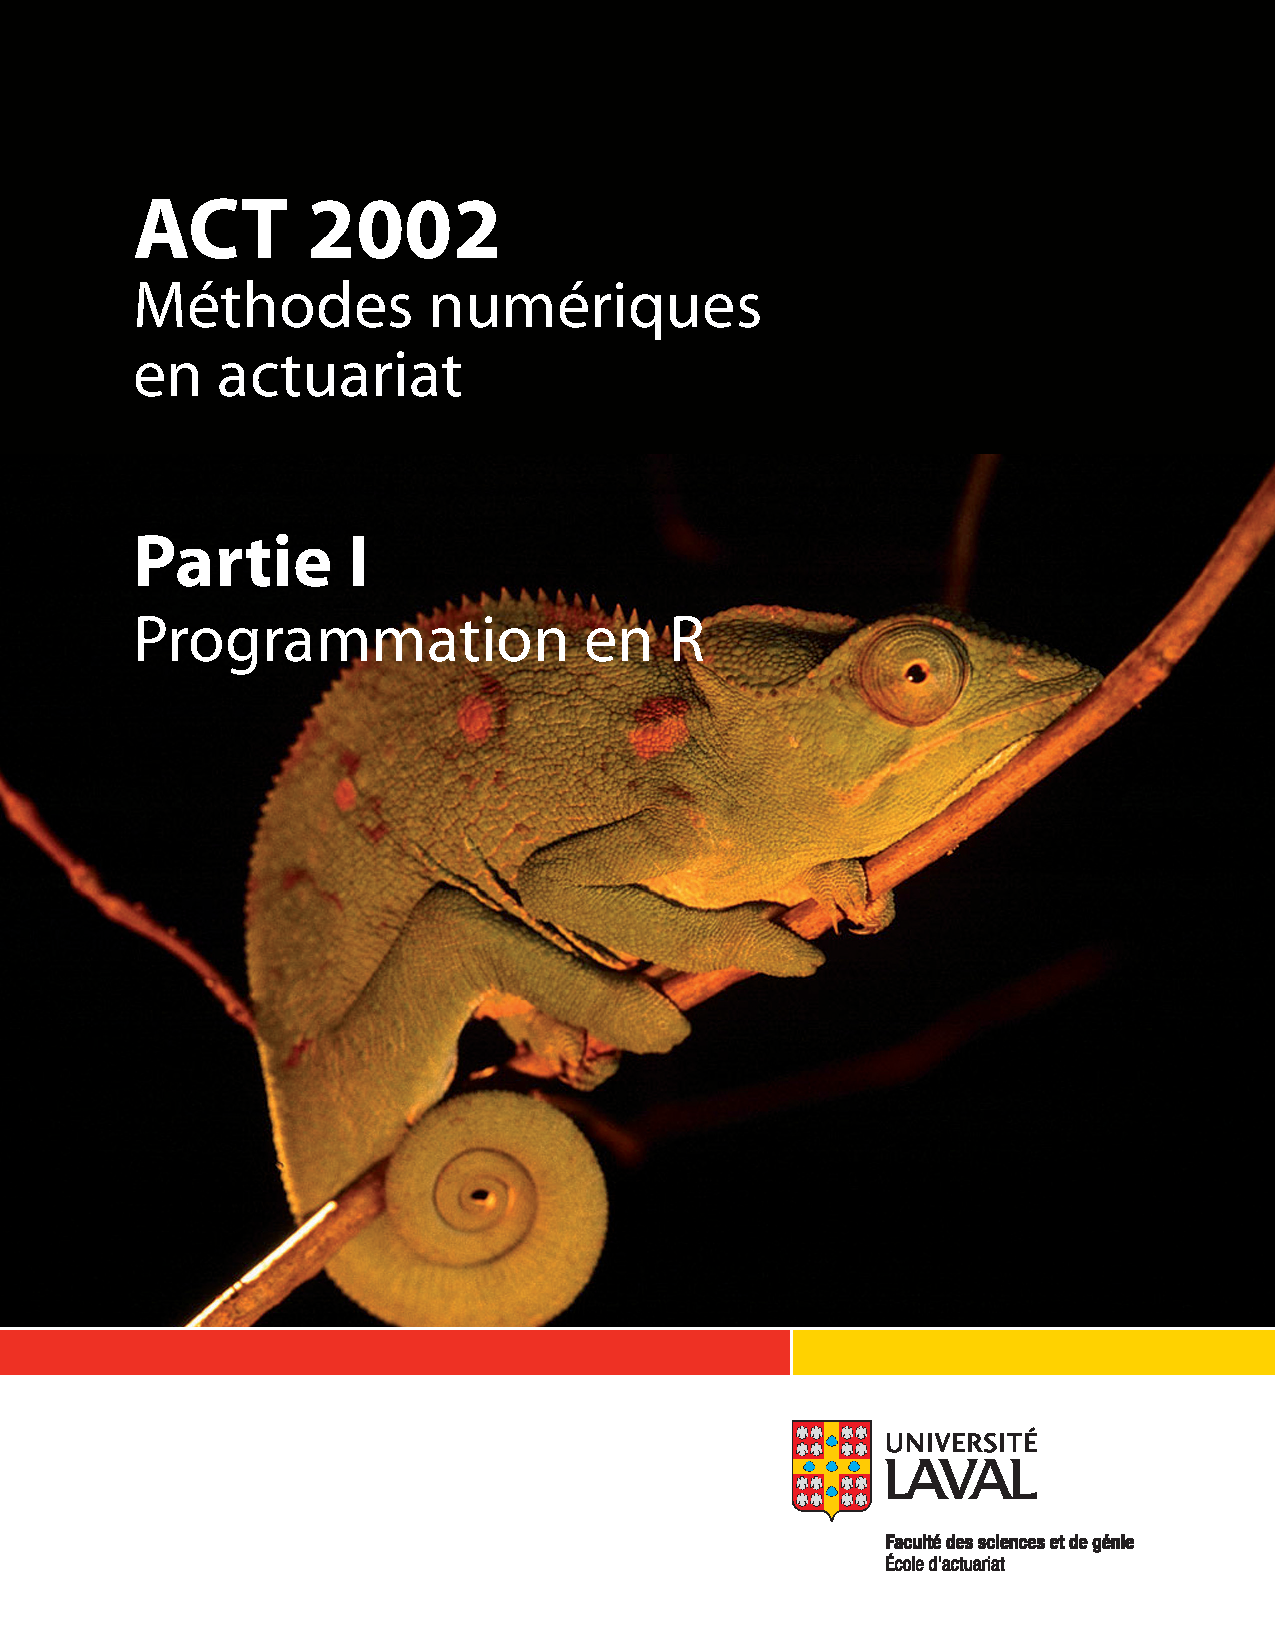
\includepdf[pages=1]{couvertures-partie_1}
\setkeys{Gin}{width=0.8\textwidth}
\cleardoublepage

\begin{adjustwidth*}{-12mm}{-72mm}
  \sffamily
  \raggedright
  \vspace*{-17mm}
  \thetitle \\
  \vspace*{20mm}
  \theparttitle \\
  \vspace*{32mm}
  \theauthor \\
  \vspace*{\fill}
  \thedate
\end{adjustwidth*}

%%% Local Variables:
%%% mode: latex
%%% TeX-master: "methodes_numeriques-partie_3"
%%% coding: utf-8
%%% End:

\clearpage

\begingroup
\calccentering{\unitlength}
\begin{adjustwidth*}{\unitlength}{-\unitlength}
  \setlength{\parindent}{0pt}
  \setlength{\parskip}{\baselineskip}

  {\textcopyright} {\year} Vincent Goulet \\

  
\includegraphics[height=7mm,keepaspectratio=true]{../share/by-sa}\\%
Cette création est mise à disposition selon le contrat
\href{http://creativecommons.org/licenses/by-sa/4.0/deed.fr}{%
  Attribution-Partage dans les mêmes conditions 4.0 International} de
Creative Commons. En vertu de ce contrat, vous êtes libre de:
\begin{itemize}
\item \textbf{partager} --- reproduire, distribuer et communiquer
  l'{\oe}uvre;
\item \textbf{remixer} --- adapter l'{\oe}uvre;
\item utiliser cette {\oe}uvre à des fins commerciales.
\end{itemize}
Selon les conditions suivantes:

\begin{tabularx}{\linewidth}{@{}lX@{}}
  \raisebox{-9mm}[0mm][13mm]{%
    
\includegraphics[height=11mm,keepaspectratio=true]{../share/by}} &
  \textbf{Attribution} --- Vous devez créditer l'{\oe}uvre, intégrer
  un lien vers le contrat et indiquer si des modifications ont été
  effectuées à l'{\oe}uvre. Vous devez indiquer ces informations par
  tous les moyens possibles, mais vous ne pouvez suggérer que
  l'Offrant vous soutient ou soutient la façon dont vous avez utilisé
  son {\oe}uvre. \\
  \raisebox{-9mm}{
\includegraphics[height=11mm,keepaspectratio=true]{../share/sa}}
  & \textbf{Partage dans les mêmes conditions} --- Dans le cas où vous
  modifiez, transformez ou créez à partir du matériel composant
  l'{\oe}uvre originale, vous devez diffuser l'{\oe}uvre modifiée dans
  les même conditions, c'est à dire avec le même contrat avec lequel
  l'{\oe}uvre originale a été diffusée.
\end{tabularx}


  \textbf{Code source} \\
  Le code source {\LaTeX} et R de ce document est disponible à l'adresse
    \url{https://svn.fsg.ulaval.ca/svn-pub/vgoulet/documents/methodes_numeriques/}
  ou en communiquant directement avec l'auteur.

  \textbf{Couverture} \\
  Le reptile en couverture est un caméléon tapis (\emph{Furcifer
    lateralis}) originaire de Madagascar. Adulte, sa taille atteint
  les 25~cm, queue comprise.

  Crédit photo: Michabln Schwarz; \url{http://fc-foto.de/2077174}
\end{adjustwidth*}
\endgroup

%%% Local Variables:
%%% mode: latex
%%% TeX-master: "methodes_numeriques-partie_4"
%%% coding: utf-8
%%% End:

\clearpage

\pagestyle{companion}

\chapter*{Introduction}
\addcontentsline{toc}{chapter}{Introduction}
\markboth{Introduction}{Introduction}

Il existe de multiples ouvrages traitant de l'environnement
statistique R. Dans la majorité des cas, toutefois, le logiciel est
présenté dans le cadre d'applications statistiques spécifiques. Ce
document se concentre plutôt sur l'apprentissage du langage de
programmation sous-jacent aux diverses fonctions statistiques, langage
lui aussi nommé R.

Chaque chapitre présente en rafale plusieurs éléments de théorie avec
généralement peu d'exemples. La lecture d'un chapitre permet donc
d'acquérir rapidement plusieurs nouvelles connaissances sur le langage
R. Cependant, pour compléter son apprentissage, le lecteur devra aussi
étudier attentivement et, surtout, exécuter ligne par ligne le code R
fourni dans les sections d'exemples à la fin des chapitres (sauf un).
Ces sections d'exemples couvrent l'essentiel des concepts présentés
dans les chapitres et les complémentent souvent. L'étude de ces
sections fait partie intégrante de l'apprentissage du langage R.

Le code des sections d'exemples est disponible dans le site du cours.
Nous fournissons également des fichiers de sortie contenant les
résultats de chacune des expressions.

Un symbole de lecture vidéo dans la marge, tel que ci-contre, indique
qu'une capsule vidéo sur \capsule{le sujet} identifié par la marque de
soulignement est disponible dans le site du cours.

Certains exemples et exercices font référence à des concepts de base
de la théorie des probabilités et des mathématiques financières. Les
contextes actuariels demeurent néanmoins peu nombreux et ne devraient
généralement pas dérouter le lecteur pour qui ces notions sont moins
familières. Les réponses de tous les exercices se trouvent en annexe.

On trouvera également en annexe une brève introduction à l'éditeur de
texte GNU~Emacs et au mode ESS, ainsi qu'une présentation sur
l'administration d'une bibliothèque de packages R.

Je tiens à remercier M.~Mathieu Boudreault pour sa collaboration
dans la rédaction des exercices.

%%% Local Variables:
%%% mode: latex
%%% TeX-master: "methodes_numeriques-partie_1"
%%% coding: utf-8
%%% End:


\cleartorecto
\tableofcontents*

%% Vignette tirée de xkcd.com
\cleartoverso
\thispagestyle{empty}
\begin{vplace}[0.45]
  \centering
  \setkeys{Gin}{width=\textwidth}
  \begin{minipage}{351pt}
    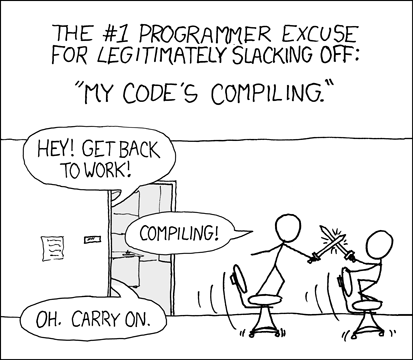
\includegraphics{compiling.png} \\
    \footnotesize\sffamily%
    Tiré de \href{http://xkcd.com/303/}{XKCD.com}
  \end{minipage}
  \setkeys{Gin}{width=0.8\textwidth}
\end{vplace}

\mainmatter

\include{presentation}
\include{bases}
\include{operateurs}
\include{exemples}
\include{fonctions}
\include{avance}

\appendix
\include{emacs+ess}
\include{packages}
\chapter{Réponses des exercices}
\label{reponses}
\markboth{Réponses des exercices}{Réponses des exercices}

\input{solutions-bases}
\input{solutions-operateurs}
\input{solutions-exemples}
\input{solutions-fonctions}
\input{solutions-avance}

%%% Local Variables:
%%% mode: latex
%%% TeX-master: "methodes_numeriques-partie_1"
%%% coding: utf-8
%%% End:
     % différent de Introduction à la...

\bibliography{r,stat,informatique}

\cleardoublepage
\printindex

\cleartoverso

\thispagestyle{empty}
\vspace*{\fill}

\begingroup
\calccentering{\unitlength}
\begin{adjustwidth*}{\unitlength}{-\unitlength}
  \begin{flushleft}
    \small %
    Ce document a été produit avec le système de mise en page
    {\XeLaTeX}. Le texte principal est en Lucida Bright~OT 11~points,
    les mathématiques en Lucida Bright Math~OT, le code informatique
    en Lucida Grande Mono~DK et les titres en Adobe Myriad~Pro. Des
    icônes proviennent de la police Font~Awesome. Les graphiques ont
    été réalisés avec R.
  \end{flushleft}
\end{adjustwidth*}
\endgroup
\vfill


\cleartoverso

%% Page couverture arrière.
\setkeys{Gin}{width=\paperwidth}
\includepdf[pages=2]{couvertures-partie_1}

\end{document}

%%% Local Variables:
%%% mode: latex
%%% TeX-engine: xetex
%%% TeX-master: t
%%% coding: utf-8
%%% End:
